% !TeX root = RJwrapper.tex
\title{SIREN: A Hybrid CFA-EFA R Package for Controlling Acquiescence in Restricted Factorial Solutions}
\author{by David Navarro-Gonzalez, Pere J. Ferrando, Fabia Morales-Vives, Ana Hernandez-Dorado}

\maketitle

\begin{abstract}
  The \pkg{siren} package implements a two-step procedure that allows restricted (confirmatory) factor analytic (FA) solutions to be fitted in data matrices that have been previously ‘cleaned’ of the biasing effects of acquiescent responding (AR) by using an unrestricted (exploratory) FA specification. So, the procedure which is implemented is hybrid: i.e. (a) an unrestricted acquiescence (ACQ) factor is first fitted to the data, (b) the residual data (or covariance) matrix after the impact of ACQ has been partialled-out is obtained, and (c) a restricted FA solution is fitted to the residual matrix. Although the basic foundations of the procedure are known, it contains new methodological developments that are, all of them, implemented in the package. So, provided that fully or partially balanced scales are available, the researcher will be able to: (a) calibrate a multidimensional CFA solution which is free from AR, (b) assess the goodness of model-data fit of this solution, and (c) obtain individual score estimates in the content as well as in the ACQ factors. The functioning of the program is assessed by means of a simulation study, and illustrated with a toy example. Its usefulness is also demonstrated by using an illustrative example in the personality domain. \pkg{siren} is submitted to be a valuable tool for use in item CFA applications when AR is expected to be operating.
\end{abstract}

\section{Introduction}

Valid interpretation of typical-response or non-cognitive (personality, attitude, interest, etc.) test scores requires that the item responses that are to be calibrated and scored meet a series of conditions. Of these, one of the more basic is that the responses truly reflect the influence of the content variables intended to be measured and are not affected by other systematic determinants unrelated to this content. In particular, this article is concerned with Acquiescent Responding (AR): the tendency to agree or endorse an item regardless of its content \citep{Messick:1966} as a response determinant. When AR is operating and is not properly controlled, a series of invalidating effects can be expected, both at the calibration level (biased item parameter estimates and spurious evidence of multidimensionality) and at the scoring level (scores that reflect a mixture of content and AR and so they cannot be univocally interpreted).

Test designers and practitioners are generally aware of the potential invalidating effects of AR, and use procedures for controlling them. Of these, the most common is to develop balanced scales. Provided that the content variables can be considered as continuous dimensions with two end poles, in a fully balanced scale half of the items are keyed toward one of the poles while the other half are keyed toward the opposite pole  \citep{Savalei:2014,Vigil-Colet:2020}.

Statistical control of AR in test designs that use balanced scales is generally based on factor analytic (FA) procedures, and essentially entails explicitly modeling AR as an additional non-content factor. This FA-based control operates at two levels \citep[see][]{Ferrando:2003}: first, at the level of the factor structure obtained in the calibration stage (thus avoiding or minimizing the invalidating effects mentioned above); and second, at the level of the factor score estimates derived from the calibration structure (thus, providing “cleaner” content score estimates that have a more univocal interpretation).

Within the general FA modeling, two main approaches exist at present  \citep{Savalei:2014,delaFuente:2020}. The first is fully confirmatory, and the solution is identified by restricting all the loadings on the additional Acquiescence (ACQ) factor to have the same unit value  \citep{Billiet:2000}. The second is exploratory or semi-confirmatory ( \citep{Ferrando:2003}): First, (a) an unrestricted ACQ factor with (possibly) different loadings and (b) an also unrestricted (EFA) direct “content” solution are obtained. Second, the direct content solution is either analytically rotated (fully exploratory solution) or rotated against a specified or semi-specified target (semi-confirmatory solution). The pros and cons of both approaches have been discussed and compared by \citet{Savalei:2014} and \citet{delaFuente:2020}. Both studies concluded that the confirmatory approach is more robust and user-friendly than the EFA with target rotation. However, it is also more sensitive to violation of the unit-weight loading assumption for the ACQ factor.

Within the general FA-based controlling procedure, two main approaches exist at present \citep{Savalei:2014,delaFuente:2020}. The first is fully confirmatory, and, in it, the structural FA solution is identified by restricting all the loadings on the additional Acquiescence (ACQ) factor to have the same unit value  \citep{Billiet:2000}. The second is exploratory or semi-confirmatory  \citep{Ferrando:2003}: First, an unrestricted ACQ factor with (possibly) different loadings together with a direct (i.e. non-rotated) unrestricted or exploratory (EFA) “content” solution are obtained. Second, the direct content solution is either analytically rotated (in a fully exploratory solution) or rotated against a specified or semi-specified target (in a semi-confirmatory solution). The pros and cons of both approaches have been discussed by \citet{Savalei:2014} and \citet{delaFuente:2020}. Both studies concluded that the confirmatory approach is more robust and user-friendly than the semi-confirmatory EFA with target rotation. However, it is also more sensitive to violation of the unit-weight loading assumption for the ACQ factor.

The aim of this paper is to propose and implement a “hybrid” approach, named SIREN, that combines features of both the CFA and EFA approaches. Furthermore, the procedure is comprehensive in that it is intended for fitting multiple content solutions and can also be used with scales that are not fully balanced (see below). Because we are using the same name for the proposed procedure and the package that implements it, in the remainder of the paper, we shall use the distinction “SIREN procedure” and “\pkg{siren} package” when necessary so as to avoid confusion.

Most of the basic foundations of SIREN have been discussed in the FA literature \citep[e.g.][]{Nunnally:1978}. Furthermore, the approach we shall propose is multi-step (see below), and the first step: estimating an unrestricted ACQ factor, is, essentially, the same as that used in the exploratory/semi-confirmatory approaches summarized below. So, this part of the proposal will not be discussed in detail but relevant references will be provided to the interested reader. On the other hand, the full proposal contains new developments, and these are the ones that will be discussed here in more detail.

\subsection{Basic general results and rationale of the proposal}

Consider a set of $n$ items intended to measure $p$ common content factors (e.g. personality dimensions). The basic FA model equation in the population is:
\begin{equation}
  \label{EQ1}
  \mathbf{Z} = \boldsymbol{\Lambda} \boldsymbol{\theta} + \boldsymbol{\Psi} \mathbf{E}
\end{equation}
where \textbf{Z} is an \textit{n × 1} random vector of observed item scores; $\boldsymbol{\Lambda}$ is an \textit{n × p} factor pattern matrix; $\boldsymbol{\theta}$ is an \textit{p × 1} random vector of ‘true’ common factor scores; $\boldsymbol{\Psi}$ is an \textit{n × n} diagonal matrix of unique-factor loadings, and \textbf{E} is an  \textit{n × 1} random vector of unique factor scores. With regards to scaling and assumed relations, the observed item scores are in reduced form (centered around the mean), the common factor scores and the unique scores are in standard scale (zero mean and unit variance), and, finally, the unique scores are assumed to be uncorrelated with the common factors and among them. In these conditions, the reproduced covariance matrix among the $n$ item scores as implied by model \eqref{EQ1} is given by the structural equation:
\begin{equation}
  \label{EQ2}
  \boldsymbol{\Sigma} = \boldsymbol{\Lambda} \boldsymbol{\Phi} \boldsymbol{\Lambda'}  + \boldsymbol{\Psi}^{2}
\end{equation}
where $\boldsymbol{\Phi}$ is \textit{p × p}  correlation matrix containing the correlations between the ‘true’ common factor scores. Generally, in the applications considered here, the \textbf{Z} scores will not only be mean-centered, but standardized scores, and so, the implied covariance matrix $\boldsymbol{\Sigma}$ in \eqref{EQ2} will be a correlation matrix.

The main difference between an unrestricted (exploratory) and a restricted (confirmatory) solution within the general model \eqref{EQ2} is in the constraints that are imposed to the pattern matrix $\boldsymbol{\Lambda}$. In an unrestricted solution, only minimal identification constraints are imposed, so that the common space: $\boldsymbol{\Lambda} \boldsymbol{\Phi} \boldsymbol{\Lambda'}$ in \eqref{EQ2} is not restricted and multiple solutions of the same type, that fit all equally well, can be obtained from each other by rotation. In a restricted solution, the number of imposed restrictions makes the specified solution $\boldsymbol{\Lambda} \boldsymbol{\Phi} \boldsymbol{\Lambda'}$ unique, in the sense that it cannot be obtained by rotation of another solution  \citep[see][]{Joreskog:1969}. Although a restricted solution can be obtained by using different sets of constraints, the most usual consist of imposing an independent-cluster structure \citep[e.g.][]{McDonald:2000}: each item has only a non-zero loading in one factor, having zero loadings in all the others.

At this point, we will start to develop a small, artificial toy example to help clarify the explanations that will follow. Suppose a questionnaire made up of 8 factorially simple items that measure two moderately correlated factors, so that the independent-cluster structure in the population is:

\begin{table}[H]
  \centering
  \caption{Toy example: restricted CFA solution with two correlated content factors.}
  \label{tab1}
  \begin{tabular}{ c c }
    $\boldsymbol{\Lambda} =  \begin{bmatrix}  \begin{array}{rr}  0.7 & 0.0 \\ -0.7 & 0.0 \\ 0.7 & 0.0 \\ -0.7 & 0.0 \\  0.0  &  0.6 \\  0.0  & -0.6 \\  0.0  &  0.6 \\  0.0  & -0.6 \end{array}\end{bmatrix}$
    &
    $\boldsymbol{\Phi} = \begin{bmatrix} \begin{array}{rr} 1.0 &  0.3 \\ 0.3 &  1.0 \end{array} \end{bmatrix}$
  \end{tabular}
\end{table}

A CFA estimation of this structure can be specified by constraining to zero the 8 elements of $\boldsymbol{\Lambda}$ that should be zero and freely estimating the remaining 8 loadings and the interfactor correlation based on the sample correlation matrix \textbf{R}. Note that, for a solution of this type to be defined, the practitioner must be able to specify first, the number of content factors that the questionnaire intends to measure (two in the example), and second, the specific items that define each factor.  Furthermore, the items are supposed to be all factorially simple, so that each item is a marker of the factor it measures and has negligible loadings on the remaining factors. These conditions are not easy to achieve, but can be feasible at advanced stages of test development.

Suppose now that the \textbf{content} structure of our example is that in \cref{tab1} but, at the same time, the item responses are also partly affected by AR, conceptualized as an additional non-content factor (see \cref{tab2} below). Now, even though the content structure was correct, if the specified two-factor structure above was directly fitted to \textbf{R}, two types of distorted results would be expected. First, the goodness of model-data fit would not be good. Second, the loading and inter-factor correlation estimates would be biased with respect to the parameter values in (2) \citep[see e.g.][]{DeMars:2014, Ferrando:2010}.

The rationale of SIREN can now be explained from the results above. At the calibration level, the basic idea is to obtain a corrected or cleaned covariance/correlation matrix $\mathbf{R}_{corr}$ in which the impact of the ACQ factor has been partialled-out. If this is done correctly, a specified restricted CFA solution can be next fitted to $\mathbf{R}_{corr}$  instead of $\mathbf{R}$. This solution will now fit well, and the ‘true’ content parameters in \cref{tab1} will be well recovered.
At the scoring level, once the ACQ and the content structures have been properly estimated, ACQ and content individual score estimates (i.e. factor scores) can be next obtained based on the unrestricted ACQ pattern and the restricted, CFA content solution.

As mentioned above, in order to control for the impact of AR, the items of the questionnaire have to be fully or partially balanced. In the present scenario, the condition of full balance implies that, within each factor, half of the items that define this factor are positively keyed and the other half are negatively keyed. The condition of partial balance implies here that all the factors contain positively and negatively keyed items, but that the number of positive and negative items is not the same at least in one factor \citep[e.g.][]{Lorenzo-Seva:2009}.

We shall now illustrate the points so far discussed with our toy example. Suppose now that the full content plus ACQ structure in the population is that in \cref{tab2}. As the content pattern loadings show, however, the practitioner has done her work well and, within each factor, the items are fully balanced:  within each content factor, half of the loadings are positive and half negative. As for the ACQ factor, (a) all the loadings are positive, and (b) they are smaller in magnitude than the content loadings. Both features are expected in empirical applications. First, AR is the tendency to agree with the item regardless of the direction in content (hence all loadings are expected to be positive). Second, in a well-designed measure, the item responses are expected to be far more determined by the content they measure than by ACQ.

\begin{table}[H]
  \caption{Toy example: complete solution when ACQ is operating. Balanced items.}
  \label{tab2}
  \centering
  \begin{tabular}{c c}
    $\boldsymbol{\Lambda} =
    \begin{bmatrix}
      \begin{array}{rrr}
        0.7  &  0.0 &  0.1 \\
        -0.7 &  0.0 &  0.2 \\
        0.7  &  0.0 &  0.3 \\
        -0.7 &  0.0 &  0.3 \\
        0.0  &  0.6 &  0.3 \\
        0.0  & -0.6 &  0.3 \\
        0.0  &  0.6 &  0.2 \\
        0.0  & -0.6 &  0.1 \\
      \end{array}
    \end{bmatrix}$
    &
    $\boldsymbol{\Phi} =
    \begin{bmatrix}
      \begin{array}{rrr}
        1.0 &  0.3 &  0.0 \\
        0.3 &  1.0 &  0.0 \\
        0.0 &  0.0 &  1.0 \\
      \end{array}
    \end{bmatrix}$
  \end{tabular}
\end{table}

Once a complete solution such as that in \cref{tab2} has been estimated, it can be next taken as a basis for obtaining ACQ and content score estimates (i.e. factor scores) for each individual. As discussed above, these scores will now be cleaner and have a more univocal interpretation.

\subsection{General description of the procedure and relation with previous approaches}

We propose a general multi-stage procedure in which the number of stages depends on whether the test is fully or only partially balanced. So, within each of the two conditions (full balance or partial balance), the stages will be described separately. Conceptually, however, it is useful to view the overall procedure as based on three general stages that are common in both conditions. In the first stage, an ACQ factor is estimated from the properties of the (partially or fully) balanced set of items, and the impact of this factor on the inter-item correlation matrix is partialled-out. In the second stage, a specified CFA solution is fitted to the ‘cleaned’ correlation matrix. Finally, in the third stage, individual score estimates are obtained from the hybrid solution (i.e. the unrestricted ACQ factor and the restricted content-factor solution).

Although the sequential rationale just described is conceptually the clearest, the structural solution at the second stage above can actually be specified and fitted in two ways. The first way directly follows from the corrected-correlation-matrix concept: to fit a CFA solution to a reduced correlation matrix which is free from ACQ. In the \pkg{siren} package, this way of fitting the model corresponds to the ‘resid’ method option (i.e. use the residual or corrected matrix as input for the CFA) as defined below. The second way is to take the estimated ACQ loadings obtained at the first stage as if they were fixed and known, and next to specify a full CFA solution that includes an additional ACQ factor with loadings fixed at the obtained values. In the \pkg{siren} package, this second choice corresponds to the ‘fixed’ method option defined below.  As we shall see, the results from both approaches must be the same. In either case, the corrected or residual correlation matrix is provided in the output of the SIREN package under the heading “rresidmatrix”.

The explanation above allows the relation between SIREN and previous approaches to be discussed in more detail. If the solution is specified in the first way above (‘resid’ method option), SIREN can be viewed as a particular application of a residual covariance analysis approach, i.e. to initially correct a covariance or a correlation matrix for unwanted effects before it is used as input for further structural analyses \citep[e.g.][] {Andrews:1984, Asparouhov:2023, DeCastellarnau:2021, tenBerge:1999}.

If the second equivalent specification above: full CFA solution that includes the additional fixed ACQ factor (‘fixed’ method option), is used instead, then SIREN can be regarded as a modification of the CFA approach initially proposed by \citet{Billiet:2000}. In effect, in the latter, the ACQ loadings are fixed all of them to unity for identification purposes (which is generally unrealistic). In contrast, in SIREN these loadings are fixed at the (possibly different) values estimated at the first stage.

\subsection{Background results and required general conditions}

Consider again a fully-balanced questionnaire made up of $n$ items (where n is even) that measure a set of (possibly related) traits $\theta_1...\theta_l...\theta_m$, so that each item is a factorially pure measure of one of the $m$ content factors plus of an acquiescence factor $\theta_a$ which is unrelated to the content factors. For an individual $i$ that responds to an item $j$ that measures content factor $l$, the structural model in a $z$-score metric (mean 0 and variance 1) is

\begin{equation}
  \label{EQ3}
  z_{ij} = \lambda_{jl}\theta_{il}+\alpha_{ja}\theta_{ia}+\varepsilon_{ij}
\end{equation}

This is a scalar specification of matrix equation \eqref{EQ1} based on an independent-cluster pattern. Only a single content loading per item is specified because the remaining content loadings are zero. The $\alpha_{ja}$ loading is the loading item $j$ has on the ACQ factor. Finally, the residual terms $\varepsilon$s have zero means, and are uncorrelated with the factors or with one another.

The $z$ item responses in \eqref{EQ3} can be treated as categorical or (approximately) continuous. In the first case, the standardized scores would correspond to the continuous-unbounded “strength” latent variable that are assumed to underlie the observed scores and generate them according to a threshold mechanism \citep[see][]{Muthen:1993}. In the second case, they are directly the standardized item scores. From this general modeling, it follows that the inter-item correlations are polychoric correlations in the first case, and product-moment correlations in the second case \citep[see e.g.][for further details]{Ferrando:2013}. In the \pkg{siren} package, the user decides how the item responses are to be treated by using the ‘corr’ argument defined below, which has two options: "Pearson" (product-moment correlations) or “Polychoric” (Polychoric/Tetrachoric correlations). Once the correlation matrix has been obtained, the results that follow are common for both treatments.

Consider now the (polychoric or product-moment) reduced inter-item correlation matrix with communalities in the main diagonal \citep[see][]{Ferrando:2010}. If (a) all the assumptions so far (independent-cluster structure, full balance within factors) were met, (b) the specified FA model was correct, and (c) the item communalities were known, then the first centroid loading \citep[e.g.][]{Lawley:1960} for item $j$ would correspond to the loading this item has on the ACQ factor (i.e. $\alpha_{ja}$) in the population. In the unidimensional content case, further details on this result can be obtained from \citet{Ferrando:2003}, and, provided that full within-factor balance applies, the result also holds directly in the multidimensional case. Indeed, the conditions above are only approximately met at best (in particular, true communalities as assumed in the centroid method, are never known; \citep[see][]{McDonald:1978}. And, furthermore, the first centroid loading is a sample estimate. For these reasons, our choice in SIREN is to first obtain the first principal-axis or canonical factor by using an efficient EFA estimation procedure: Minimum Rank Factor Analysis \citep[MRFA,][]{tenBerge:1991}, and next rotate this factor against the centroid vector that is used as a criterion \citep[see][]{Eysenck:1950}. The final factor so obtained is taken in SIREN as an estimate of the ACQ factor. As for the MRFA choice, it is because of its robustness and because it provides estimates of the proportion of common variance accounted for by the different factors, and this information is useful for assessing the relevance of the ACQ factor in terms of explained common variance. The proportion of ACQ explained common variance is provided under the heading ‘rACQvariance’ in the SIREN package output.

Provided that the preliminary general conditions discussed above are met, the correct functioning of the SIREN procedure once the ACQ factor has been partialled-out depends on two main points. The first point is of a mathematical nature, and is critical if unbiased loadings (especially those of content factors) are to be obtained. The second is of a statistical nature, and is important if the goodness-of-fit assessment needs to be correct.

Obtaining unbiased loading estimates in SIREN mainly depends on achieving full balance (either for the total test or for a core balanced set), in principle, within each factor. In more detail, what is required is that the sum of content loadings within each factor be equal to zero. If it is, then the first centroid (or MRFA factor) will reflect only AR, so partializing it from the correlation matrix will remove only this response bias and leave a 'clean' corrected correlation that will reflect only content. However, if balance is not achieved, then, to a greater or lesser extent, the first centroid factor will reflect a mixture of ACQ and content. So, some content will be removed by partializing, and the resulting content loadings will be biased \citep[see][]{tenBerge:1999}. Having said that, however, we also note that the strict condition of full balance within each factor (or the core set within each factor) is probably too strong. Preliminary results by the writers suggest that, provided that the content CFA solution is correct and full balance holds for the entire set (or core set) of items, but not necessarily for each factor, then SIREN would still perform correctly in most cases. The extent to which the content loading estimates will degrade as imbalance increases is best addressed using simulation, and this will be done in the next section.

We turn now to the second, statistical point. Our proposal can be viewed as a particular application of what \citep{Nunnally:1978} called an ad-lib factorial process, in which successive factors are fitted to residual matrices by using different methods. We consider our proposal to be indeed legitimate, however, its multi-stage nature necessarily entails a loss of information and efficiency, because the successive estimates are taken as fixed and known, and their uncertainty is not taken into account. In agreement with authors such as \citep{DeCastellarnau:2021, Nunnally:1978, tenBerge:1999} and the empirical results provided by \citep{Oberski:2013}, however, we believe that the impact of the loss of efficiency discussed above on the point estimates and indices of goodness of fit will be relatively minor in practice provided that the proposed solution is correct and the basis conditions are reasonably met. The issue, however, needs to be, and will be, assessed by using simulation.

\subsection{Multi-stage approach with fully balanced scales}

The fulfillment of the full balance condition is checked automatically by the \pkg{siren} package by using the information provided in the ‘target’ argument (described below), in which the content pattern matrix with the signed dominant loading of each item on its corresponding factor is provided as input by the user. An example of a target would be the first two columns of $\boldsymbol{\Lambda}$ in \cref{tab2}.
The specific stages in this case are:

Stage 1: for the $n$ test items, the ACQ factor loadings are estimated by: (a) obtaining the direct (canonical) MRFA solution from the inter-item correlation matrix, by specifying $m+1$ factors (b) obtaining the first centroid from the inter-item correlation matrix (to be used as criterion), and (c) rotating the MRFA solution to the position in which the first canonical MRFA factor has maximal congruence with respect to the criterion. Essentially, the process is a target rotation against a single target vector (the first centroid). However, because the canonical MRFA solution is orthogonal, the rotation is univocally defined. Finally, the criterion of maximal congruence is defined in least squares terms: i.e. the first rotated MRFA factor is that is the closest to the target centroid in the least-squares sense.

Stage 2: obtain the corrected (i.e. ACQ free) inter-item residual matrix as $\mathbf{R}_{corr}$ = $\bf{R}$ $ - \boldsymbol{\alpha}$$\boldsymbol{\alpha}^{'}$. The $\mathbf{R}_{corr}$ matrix is, and should be treated as, a residual covariance matrix (not a correlation matrix).

Stage 3: The prescribed CFA solution can be specified and fitted in two alternative ways. The first is to input $\mathbf{R}_{corr}$ specified as a covariance matrix to the SEM program, and request a standardized solution. The output will consist of the standardized content pattern with loadings that are free of ACQ. The second way is to input the raw data to the SEM program, by specifying the prescribed CFA content solution, plus an additional ACQ factor in which all the loadings are specified as fixed and known. In this second specification, the ACQ loadings $\boldsymbol{\alpha}$ obtained in stage 2 cannot be imputed directly because $\mathbf{R}_{corr}$ is a covariance matrix (i.e. unstandardized) while the loadings on $\boldsymbol{\alpha}$ are standardized. The correct values to be imputed are thus those obtained by multiplying each standardized loading on $\boldsymbol{\alpha}$  by the corresponding item standard deviation: $\boldsymbol{\alpha_{x}}$(scaled)$=\boldsymbol{\alpha_{x}}\bf{sx}$. This scaling transforms the standardized loadings $\boldsymbol{\alpha}$ into unstandardized loadings \citep[e.g.][]{Bollen:1989}. As in the first approach, a standardized solution will next be requested in the output. If this is done, the output will now  provide the standardized content pattern with loadings free from ACQ and an additional column containing the standardized ACQ loadings. Indeed, the standardized content pattern must be the same in both specifications. In the pkg {siren} programming, the CFA in stage 3 is done by using the cfa function from the \CRANpkg{lavaan} and one of the two options described above. However, of the multiple choices that the program allows for estimating the structural item content parameters, we have chosen the one that is most congruent with the previous stages. Thus, whether the variables are treated as continuous or discrete, the estimation procedure is robust ULS, in agreement with the choice of MRFA-ULS for obtaining the ACQ estimates.

Stage 4: testing model-data fit at the structural level. Again, we have made choices within \CRANpkg{lavaan} that are in accordance with the limited-information nature of the procedure as well as with the results of the simulation study. The chosen indices are: (a) the RMSR and GFI as overall measures of misfit \citep{McDonald:1995}, (b) the RMSEA as a measure of relative fit with respect to the degrees of freedom (i.e. model complexity), and (c) the CFI as a measure of comparative fit with respect to the null independence model \citep[see][for points b and c]{Tanaka:1993}. These indices are provided in the SIREN package output under the heading ‘rfit\_indices’.

Stage 5: obtaining individual score estimates. In the basic FA equation discussed above, the factor score estimates for each individual are the estimates of the ‘true’ scores $\boldsymbol{\theta}$ in \eqref{EQ1}, which, of course, are unknown.  For both, the linear and the nonlinear models, the factor score estimates are Bayes Modal a Posteriori (MAP), which, in the continuous (linear) model, are known as regression estimates. In both cases, Bayesian scoring provides finite and plausible estimates for all the respondents under study \citep[see][]{Ferrando:2016}. For each participant, the output information consists of the point estimate of his/her level on the content factors plus his/her factor score estimate on the ACQ factor. This last estimate can be interpreted as the predisposition of the individual to engage in AR. The factor score estimates are provided under the heading 'rp\_factors' (see below).

Stages 1 to 4 in the fully-balanced procedure will be now illustrated with our toy example. Furthermore, the effects of ignoring the secondary ACQ factor will be illustrated by fitting directly the content solution in table 1 to the uncorrected (i.e observed) correlation matrix. To perform the illustration, we generated a random sample of $N=500$ simulees from a population in which the complete solution in \cref{tab2} holds. The results are in \cref{tab3}.

When an operating common factor is left unmodeled, both, biased structural estimates of the remaining parameters and deterioration of the GOF indicators are expected. So, in general terms, results in \cref{tab3} are predictable. \citet{Ferrando:2010} and \citet{DeMars:2014} can be summarized as follows. With regards to bias, SIREN does a good job, and recovers quite acceptably (given both the sample and model size) all the parameters in the toy solution: content loadings, ACQ loadings, and inter-factor correlation. On the other hand, the loading estimates in the uncontrolled solution tend to be slightly more biased, and the inter-factor correlation slightly over-estimated. In terms of GOF, that of the SIREN solution is almost perfect by all standards, which is only to be expected, as the specified solution is correct. The GOF of the uncorrected solution, however, clearly deteriorates. The amount of misfit is not terribly bad here, which is also expected in such a small model. In a larger-sized example, however, the deterioration of fit would have been much stronger.

\begin{table}[H]
  \centering
  \caption{Toy Example Results}
  \label{tab3}
  \begin{tabular}{cc}
    \hline
    Siren Loadings & Direct Loadings\\
    \hline
    \\
    $\boldsymbol{\Lambda} =
    \begin{bmatrix}
      \begin{array}{rrr}
        0.758  &  0.000  &  0.118\\
        -0.664 &  0.000  &  0.175\\
        0.620  &  0.000  &  0.311\\
        -0.723 &  0.000  &  0.257\\
        0.000  &  0.605  &  0.382\\
        0.000  & -0.583  &  0.272\\
        0.000  &  0.681  &  0.137\\
        0.000  & -0.582  &  0.165\\
      \end{array}
    \end{bmatrix}$ &
    $\boldsymbol{\Lambda} =
    \begin{bmatrix}
      \begin{array}{rr}
        0.761  &  0.000 \\
        -0.693 &  0.000 \\
        0.631  &  0.000 \\
        -0.727 &  0.000 \\
        0.000  &  0.549 \\
        0.000  & -0.552 \\
        0.000  &  0.720 \\
        0.000  & -0.586 \\
      \end{array}
    \end{bmatrix}$ \\ \\
    \hline
    Siren Phi Matrix & Direct Phi Matrix\\
    \hline
    \\
    $\boldsymbol{\Phi} = \begin{bmatrix}
      1 & .33 & 0  \\
      .33 & 1 & 0  \\
      0 & 0 & 1\\
    \end{bmatrix}$ &
    $\boldsymbol{\Phi} = \begin{bmatrix}
      1 & .35  \\
      .35 & 1  \\
    \end{bmatrix}$ \\
    \\
    \hline
    Siren GOF & Direct GOF\\
    \hline
    \\
    \begin{tabular}[t]{r@{\hspace{1mm}}l}
      CFI & = 1 \\
      GFI & = .998 \\
      RMSEA & = 0 \\
      SRMR & = .024 \\
    \end{tabular} &
    \begin{tabular}[t]{r@{\hspace{1mm}}l}
      CFI & = .922 \\
      GFI & = .974 \\
      RMSEA & = .088 \\
      SRMR & = .049 \\
    \end{tabular} \\
    \\
    \hline
    \noalign{\smallskip}
    \multicolumn{2}{l}{Note: GOF=Goodness of Fit Indices}
  \end{tabular}
\end{table}

\subsection{Multi-stage approach with partially balanced scales}

The basic idea in this case is to first obtain a fully balanced sub-set of items, which we shall denote as the core set, and estimate the ACQ loadings of the items belonging to this core by using the procedure described above. Next, the ACQ loadings of the remaining items are estimated by using a type of extension analysis based on the method of moments. Once the ACQ loading estimates are available for all the test items, the rest of the procedure can be carried out exactly as in the fully balanced case. So, the only two points that require specific discussion are: first, how to determine which items will be included in the core set, and second, how the ACQ loadings of the remaining items will be determined.

Stage 1: Choosing the core set. Within each specified factor, the positive and negative items, as specified in the ‘target’ argument are separated into two groups, and a centroid FA is performed separately in each of the two resulting inter-item correlation matrices. The loadings in the smaller set (usually that containing the negative items) are taken as fixed, and each of them is paired with the positive loading with the most similar value. The aim is for the absolute value of the sums of the positive and negative loadings to be as similar as possible. The rationale is that the effect of ACQ will be in the same direction if items are all worded in the same direction (i. e. both the positive and the negative loadings will be upwardly biased).

Stage 2: For the $n_c$ items in the core subset, the loadings on the ACQ factor are estimated using the procedure described in the fully balanced case.

Stage 3: Denote by $X_o$ an item outside the core set, and let $j=1,\cdots n_c$  be the items in the core. Let $\sum_{j=1}^{n_c}r_{oj}$ be the sum of the correlations of item $X_o$ with the remaining items in the core set (see \eqref{EQ5} for deriving these correlations). If the core items are balanced, all the terms involving the sum of content loadings will vanish, and it will then follow that  then follows that
\begin{equation}
  \label{EQ4}
  \sum_{j=1}^{n_c}r_{oj}=\alpha_{oa}\sum_{j=1}^{n_c}\alpha_{ja}
\end{equation}
So
\begin{equation}
  \label{EQ5}
  \alpha_{oa}=\frac{\sum_{j=1}^{n_c}r_{oj}}{\sum_{j=1}^{n_c}\alpha_{ja}}
\end{equation}
In words, if full balance holds for the core set, then the quotient between (a) the sum of correlations of item $X_o$ with the remaining items in the core set, and (b) the sum of ACQ loadings in the core set provides a simple estimate of the loading of item $X_o$ on the ACQ factor. Note that the sum in the denominator of \eqref{EQ5} is taken as fixed and known and has been obtained in Stage 2 above. The estimate described above can be viewed as an extension-analysis estimate \citep[e.g.][]{McDonald:1978} obtained by the method of moments.

The extension estimate \eqref{EQ5} is computed on an item-by-item basis for each of the items outside the core set in Stage 3. So, at the end of this stage, ACQ loading estimates are available for all the test items under study. This is the same situation as at the end of Stage 1 in the fully-balanced-case approach. Therefore, from this point on, the procedure is the same in both cases.

In closing this section, it is important to note that the \pkg{siren} package automatically detects if the scales are only partially balanced through the information provided by the ‘target’ argument, and, if so, also automatically carries out the three-step procedure described in this section.

\section{The \pkg{siren} package details}

Available through CRAN, the \CRANpkg{siren} package contains one main function (and additional internal functions) called \code{acquihybrid}, which implements the procedures described in the sections above.

The function usage is the following:

\begin{example}
  acquihybrid(x, content_factors, target, corr = "Pearson", raw_data=TRUE,
  method="fixed", display = TRUE)
\end{example}

in which the arguments are:

\code{x}, raw sample item scores or a covariance/correlation matrix, as a data.frame or a numerical matrix,

\code{content\_factors}, the number of content factors in the CFA solution. Each factor has to be defined by at least 3 items,

\code{target}, the pattern loading target matrix, which provides the signed dominant loading (higher in absolute value) of each item on its corresponding factor. The target is only used as a reference for assessing which items have significant loadings on which factors. The specific loading estimates are not used,

\code{corr}, determines the type of matrices to be used in the factor analysis. "Pearson": Computes Pearson inter-item correlation matrices (linear FA model); "Polychoric": Computes Polychoric/Tetrachoric inter-item correlation matrices (non-linear FA/graded model),

\code{raw\_data}, logical argument, if TRUE, the entered data will be treated as raw item scores (default). If FALSE, the entered data will be treated as an inter-item covariance/correlation matrix,

\code{method}, two choices are provided: fixed, which uses the ACQ loadings obtained in the first step to specify the ACQ factor in the CFA solution based on the raw scores, and resid, which uses the ACQ-free corrected covariance matrix as input for the CFA,

\code{display}, determines if the output will be displayed in the console, TRUE by default. If it is TRUE, the output is printed in the console and if it is FALSE, the output is returned silently to the output variable.

The data provided should be a data frame or a numerical matrix for input vectors and matrices, character variables for \code{corr} and method arguments, and logical values for \code{raw\_data} and \code{display} arguments.

The \code{acquihybrid} function returns a list variable, containing the following variables:

\code{rloadings}, the factor loadings for each content factor and acquiescence factor.

\code{rfactor\_cor}, content factor correlations.

\code{rfit\_indices}, a sub-list including a variety of popular fit indices as described above.

\code{rACQ\_variance}, the amount of common variance explained by ACQ.

\code{rresid\_matrix}, residual matrix after partialling-out for ACQ.

\code{rpfactors}, factor scores for each participant.

The package includes a detailed vignette titled “siren-vignette”, which provides step-by-step explanations of how to use the package, as well as guidance on interpreting the data. The vignette uses the same dataset as the illustrative example below.
The vignette is accessible through:

\code{vignette("siren-vignette")}

\section{Simulation studies}

To assess the behavior of the proposal under favorable conditions (correct population model) and its robustness against slight misspecifications, we conducted a simulation study which focused on both the recovery of the ‘true’ loadings in the ACQ and the content factors, and the goodness of fit results.

\subsection{Method}

A bidimensional content model with an additional ACQ factor (see Equation 1) was generated under the following specifications: (a) all the factors were orthogonal (this choice was made for simplicity); (b) the content factors contained positive and negative loadings (representing the positively and negatively keyed items); and (c) the loadings on the ACQ factor were all positive. Referring to Equation 1, the structure of the simulated model can be understood, as it defines how the observed scores are reproduced from the common factors and unique loadings, facilitating the interpretation of the factor analysis results. The number of items per factor was 10, and the sample size was fixed to 300, a value slightly higher than recommended to find accurate factor loadings estimates \citep{Fabrigar:1999}. To help the reader to visually understand the design of the simulation study, we provide a simplified version of the path diagram in \cref{fig:1}.

\begin{figure}[h]
  \centering
  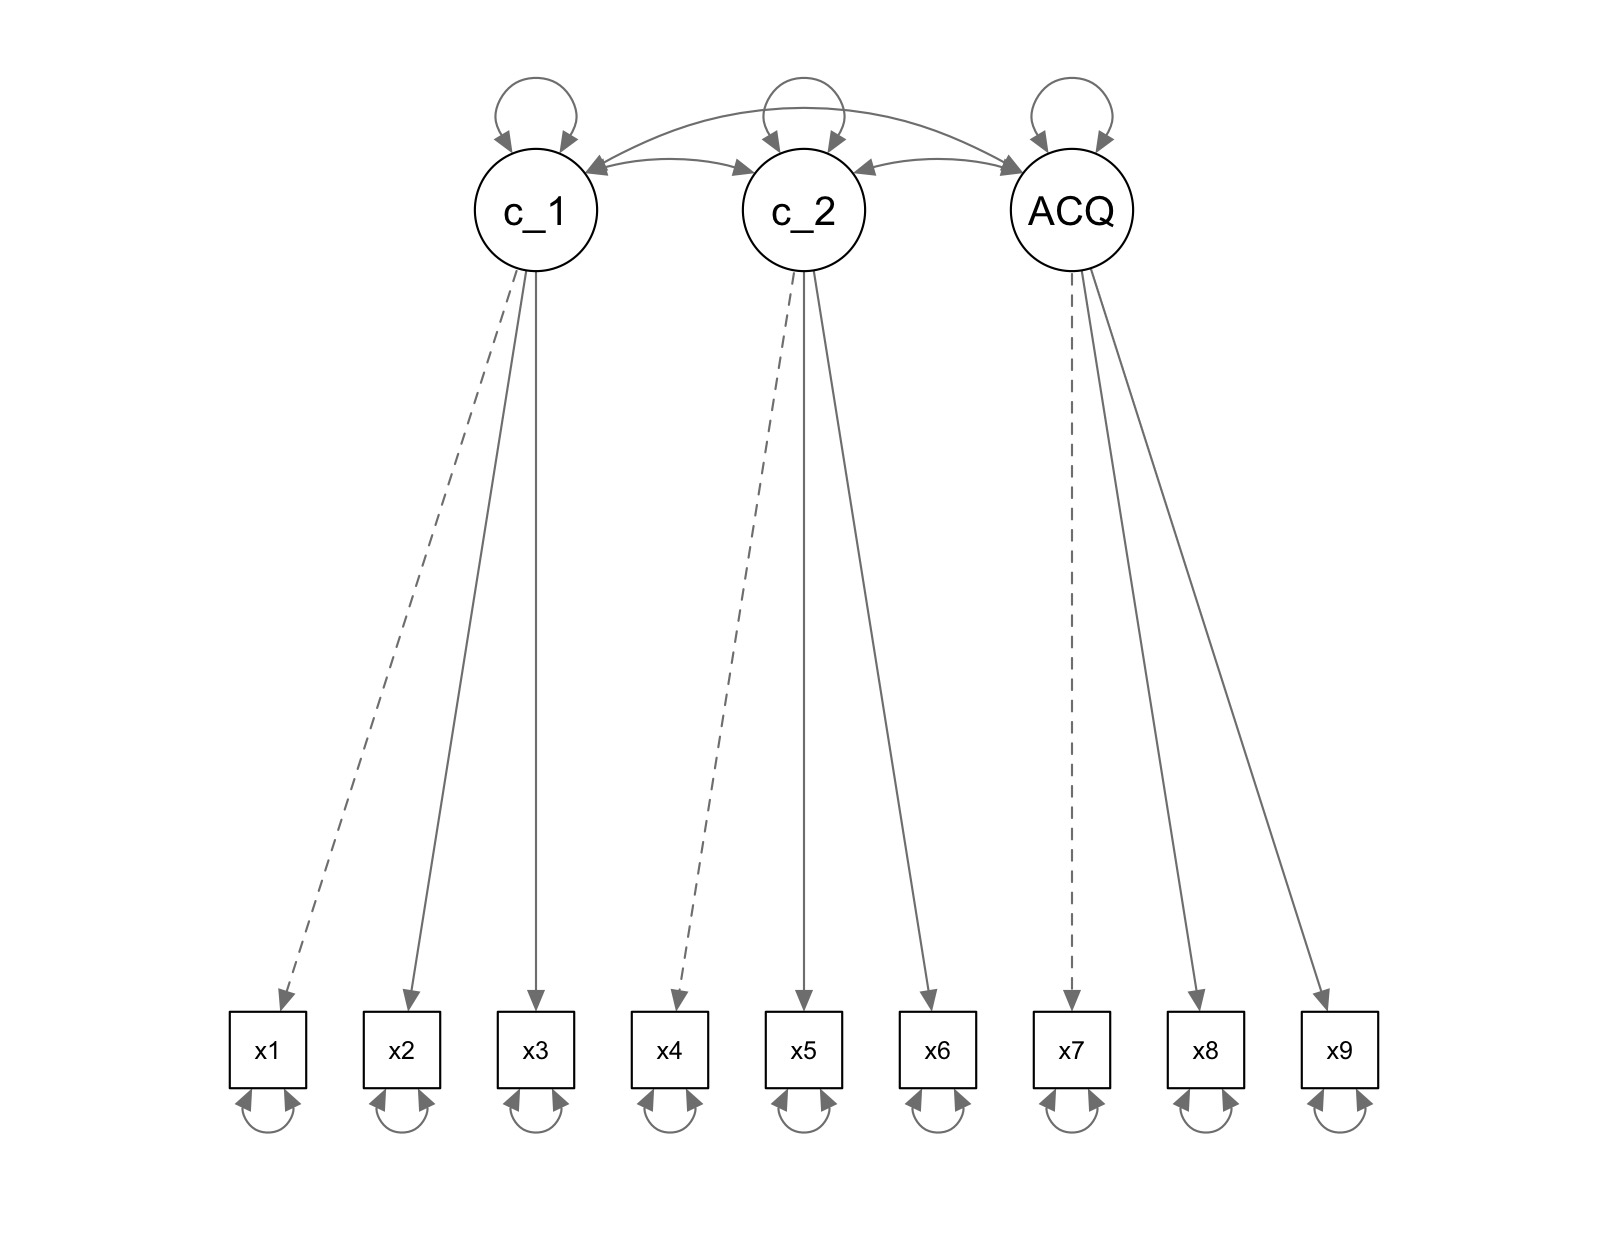
\includegraphics[width=0.8\textwidth]{toyimage.jpeg}
  \caption{Simplified version of the path diagram of the simulated model.}
  \label{fig:1}
\end{figure}

In the content factors, the simulated loadings had an average value of .6 (in absolute value) and a standard deviation of 0.1. For the ACQ factor the mean loading value was .2. The behavior of \pkg{siren} was assessed under three general conditions: (1) type of item: ordinal (four categories; FA based on polychoric correlations), or continuous (FA based on Pearson correlations); (2) pattern of substantive loadings at three levels: (a) completely balanced, (b)  60\% of positive items, and (c) 70\% of positive items; and (3) ACQ pattern at three levels: (a) equal ACQ loadings, (b) low heterogeneity (standard deviation of .01), and (c) high heterogeneity (standard deviation of .1). Thus, a factorial design with 18 experimental conditions (2 x 3 x 3) was used. These conditions were chosen according to (a) the most problematic conditions for the alternative method discussed above, and (b) the degree of realism in the applied context.

For each experimental condition, 200 replicas were generated. A higher number of replicas would simply increase the estimation time without changing the results. All analyses were conducted with R \citep{RCore:2024}. The quality of the estimates was assessed using the average bias \eqref{EQ6}
\begin{equation}
  \label{EQ6}
  \text{Average Bias} = \frac{1}{n} \sum_{i=1}^{n} (\theta_i - \hat{\theta}_i)
\end{equation}
where \( \theta_i \) are the observed or true values, \( \hat{\theta}_i \) are the predicted or estimated values, and \( n \) is the total number of observations; and the consistency of the model-data fit results was assessed using an analysis of variance (ANOVA) for each fit index considered in the study (CFI, GFI, RMSR and RMSEA).

\subsection{Results}

The results for the average bias were very stable in all conditions (see Tables \ref{tab4} and \ref{tab5}). The loadings on content factors are recovered more accurately than the loadings on the ACQ factor. In the content factors, the bias is evenly distributed across both factors, and never exceeds .05 (continuous condition) or .04 (ordinal condition) in absolute value. In contrast, the average bias in the ACQ factor is greater in the ordinal case.

No significant changes are observed when imbalance increases. However, a slight increase in bias can be noticed in those conditions in which the ACQ pattern is more heterogeneous. This increase, however, does not substantially impact the average bias of the ACQ factor (\cref{tab5}). The bias in ACQ remains at around .06, with a maximum of .077.

\begin{sidewaystable}
  \centering
  \caption{\label{tab4} Average biases of the content factor loadings}
  \begin{tabular}{ l l l l l l l l l l l l l l l l l l l l l l}
    \hline\noalign{\smallskip}
    &  &  \multicolumn{10}{c}{factor 1} & \multicolumn{10}{c}{factor 2}\\
    \hline\noalign{\smallskip}
    \multicolumn{2}{c}{Continuous} & 1 & 2 & 3 & 4 & 5 & 6 & 7 & 8 & 9 & 10 & 11 & 12 & 13 & 14 & 15 & 16 & 17 & 18 & 19 & 20 \\
    \hline
    \noalign{\smallskip}
    Bal & EQ & .047 & .044 & .045 & .047 & .045 & .043 & .045 & .042 & .04 & .041 & .044 & .043 & .042 & .046 & .045 & .046 & .041 & .049 & .042 & .044 \\
    Bal & LH & .047 & .044 & .045 & .047 & .045 & .043 & .045 & .042 & .046 & .041 & .047 & .043 & .044 & .043 & .045 & .043 & .041 & .046 & .04 & .041 \\
    Bal & HH & .046 & .043 & .047 & .047 & .045 & .044 & .045 & .045 & .043 & .044 & .045 & .046 & .04 & .046 & .043 & .043 & .044 & .05 & .045 & .042 \\
    \hline
    \noalign{\smallskip}
    LU & EQ & .04 & .044 & .047 & .044 & .043 & .046 & .044 & .042 & .043 & .043 & .04 & .043 & .045 & .045 & .045 & .042 & .043 & .044 & .042 & .043 \\
    LU & LH & .044 & .046 & .043 & .044 & .044 & .043 & .046 & .043 & .043 & .045 & .045 & .041 & .041 & .039 & .043 & .042 & .043 & .043 & .043 & .042 \\
    LU & HH & .043 & .043 & .038 & .043 & .043 & .046 & .043 & .042 & .046 & .05 & .046 & .044 & .045 & .044 & .042 & .044 & .042 & .043 & .041 & .039 \\
    \hline
    \noalign{\smallskip}
    HU & EQ & .044 & .047 & .041 & .041 & .048 & .046 & .045 & .042 & .049 & .05 & .044 & .046 & .044 & .045 & .044 & .046 & .046 & .049 & .041 & .046 \\
    HU & LH & .043 & .045 & .046 & .045 & .045 & .041 & .045 & .04 & .043 & .045 & .048 & .045 & .046 & .043 & .048 & .04 & .043 & .045 & .043 & .045 \\
    HU & HH & .05 & .044 & .046 & .045 & .047 & .043 & .044 & .047 & .05 & .049 & .046 & .049 & .042 & .048 & .046 & .047 & .049 & .045 & .044 & .046 \\
    \hline
    \noalign{\smallskip}
    \multicolumn{2}{c}{Ordinal} & 1 & 2 & 3 & 4 & 5 & 6 & 7 & 8 & 9 & 10 & 11 & 12 & 13 & 14 & 15 & 16 & 17 & 18 & 19 & 20 \\
    \hline
    \noalign{\smallskip}
    Bal &EQ & .04 & .036 & .036 & .039 & .039 & .038 & .036 & .037 & .035 & .041 & .038 & .039 & .037 & .038 & .035 & .035 & .036 & .04 & .037 & .031 \\
    Bal & LH & .04 & .036 & .036 & .039 & .039 & .038 & .036 & .037 & .035 & .041 & .039 & .042 & .037 & .036 & .035 & .034 & .038 & .039 & .037 & .034 \\
    Bal & HH & .036 & .036 & .036 & .038 & .034 & .037 & .037 & .037 & .036 & .036 & .037 & .035 & .036 & .04 & .04 & .037 & .037 & .038 & .038 & .037 \\
    \hline
    \noalign{\smallskip}
    LU & EQ & .039 & .035 & .037 & .04 & .034 & .038 & .035 & .035 & .033 & .036 & .032 & .038 & .038 & .035 & .036 & .036 & .04 & .035 & .037 & .037 \\
    LU & LH & .039 & .034 & .038 & .038 & .037 & .037 & .037 & .034 & .04 & .039 & .04 & .037 & .035 & .033 & .039 & .034 & .036 & .037 & .039 & .034 \\
    LU & HH & .037 & .037 & .039 & .04 & .036 & .038 & .034 & .037 & .038 & .039 & .035 & .037 & .037 & .037 & .04 & .04 & .037 & .036 & .037 & .033 \\
    \hline
    \noalign{\smallskip}
    HU & EQ & .036 & .036 & .031 & .039 & .037 & .037 & .036 & .041 & .039 & .037 & .035 & .04 & .037 & .033 & .036 & .035 & .038 & .044 & .04 & .042 \\
    HU & LH & .037 & .038 & .036 & .04 & .037 & .035 & .036 & .036 & .041 & .038 & .036 & .038 & .035 & .035 & .041 & .037 & .036 & .036 & .039 & .039 \\
    HU & HH & .038 & .037 & .033 & .042 & .038 & .038 & .039 & .036 & .035 & .038 & .04 & .04 & .039 & .038 & .038 & .043 & .035 & .038 &0.037 & .038 \\
    \hline
    \noalign{\smallskip}
    \multicolumn{22}{l}{Note: Bal = Balanced; LU = Low Unbalanced; HU = High Unbalanced, EQ = equal; LH = Low Heterogeneity, HH = High Heteregeneity}
  \end{tabular}

\end{sidewaystable}

\begin{sidewaystable}
  \centering
  \caption{\label{tab5} Average biases of the ACQ factor loadings}
  \begin{tabular}{ l l l l l l l l l l l l l l l l l l l l l l}
    \hline\noalign{\smallskip}
    &  &  \multicolumn{10}{c}{factor 1} & \multicolumn{10}{c}{ACQ factor}\\
    \hline\noalign{\smallskip}
    \multicolumn{2}{c}{Continuous} & 1 & 2 & 3 & 4 & 5 & 6 & 7 & 8 & 9 & 10 & 11 & 12 & 13 & 14 & 15 & 16 & 17 & 18 & 19 & 20 \\
    \hline
    \noalign{\smallskip}
    Bal & EQ & .063 & .066 & .064 & .074 & .068 & .064 & .063 & .066 & .068 & .064 & .07 & .068 & .071 & .064 & .064 & .075 & .076 & .074 & .068 & .068 \\
    Bal & LH & .07 & .069 & .072 & .072 & .066 & .075 & .063 & .068 & .072 & .073 & .068 & .066 & .063 & .068 & .068 & .067 & .065 & .067 & .068 & .067 \\
    Bal & HH & .063 & .057 & .058 & .06 & .061 & .061 & .064 & .062 & .061 & .06 & .061 & .063 & .065 & .065 & .064 & .064 & .062 & .063 & .065 & .066 \\
    \hline
    \noalign{\smallskip}
    LU & EQ & .058 & .059 & .059 & .056 & .058 & .059 & .058 & .066 & .064 & .064 & .061 & .064 & .058 & .061 & .064 & .061 & .068 & .068 & .063 & .07 \\
    LU & LH & .059 & .061 & .06 & .057 & .066 & .06 & .061 & .059 & .062 & .072 & .066 & .063 & .06 & .063 & .065 & .062 & .061 & .069 & .066 & .064 \\
    LU & HH & .067 & .058 & .063 & .059 & .056 & .056 & .059 & .062 & .061 & .06 & .061 & .063 & .056 & .056 & .059 & .054 & .063 & .054 & .056 & .059 \\
    \hline
    \noalign{\smallskip}
    HU & EQ & .068 & 0.071 & 0.061 & 0.066 & .065 & .059 & .063 & 0.062 & .07 & .07 & .072 & .066 & .064 & .067 & .077 & .076 & .072 & .066 & .068 & .066 \\
    HU & LH & .063 & .058 & .066 & .063 & .064 & .061 & .068 & .071 & .068 & .075 & .071 & .068 & .069 & .063 & .071 & .068 & .074 & .064 & .068 & .067 \\
    HU & HH & .062 & .062 & .064 & .068 & .059 & .062 & .063 & .067 & .071 & .065 & .066 & .071 & .056 & .056 & .071 & .065 & .071 & .067 & .067 & .059 \\
    \hline
    \noalign{\smallskip}
    \multicolumn{2}{c}{Ordinal} & 1 & 2 & 3 & 4 & 5 & 6 & 7 & 8 & 9 & 10 & 11 & 12 & 13 & 14 & 15 & 16 & 17 & 18 & 19 & 20 \\
    \hline
    \noalign{\smallskip}
    Bal & EQ & .069 & .075 & .072 & .067 & .074 & .075 & .079 & .076 & .074 & .073 & .071 & .077 & .078 & .076 & .069 & .077 & .074 & .068 & .074 & .071 \\
    Bal & LH & .075 & .076 & .078 & .07 & .079 & .08 & .078 & .079 & .069 & .083 & .072 & .077 & .079 & .072 & .078 & .076 & .071 & .076 & .076 & .071 \\
    Bal & HH & .059 & .065 & .068 & .073 & .072 & .066 & .065 & .066 & .07 & .071 & .065 & .073 & .067 & .071 & .068 & .065 & .069 & .064 & .07 & .066 \\
    \hline
    \noalign{\smallskip}
    LU & EQ & .069 & .062 & .067 & .07 & .069 & .072 & .073 & .073 & .076 & .07 & .07 & .066 & .069 & .068 & .071 & .072 & .079 & .072 & .071 & .072 \\
    LU & LH & .073 & .061 & .074 & .071 & .074 & .073 & .068 & .076 & .073 & .065 & .069 & .076 & .065 & .073 & .073 & .074 & .075 & .072 & .072 & .075 \\
    LU & HH & .064 & .069 & .071 & .065 & .072 & .072 & .074 & .068 & .073 & .076 & .067 & .068 & .063 & .068 & .067 & .07 & .078 & .06 & .069 & .064 \\
    \hline
    \noalign{\smallskip}
    HU & EQ & .076 & .071 & .067 & .073 & .07 & .074 & .073 & .08 & .069 & .089 & .081 & .075 & .078 & .075 & .073 & .077 & .076 & .085 & .074 & .074 \\
    HU & LH & .072 & .069 & .07 & .077 & .078 & .068 & .068 & .086 & .079 & .078 & .078 & .077 & .074 & .081 & .074 & .08 & .077 & .083 & .082 & .083 \\
    HU & HH & .06 & .069 & .073 & .074 & .07 & .071 & .076 & .078 & .077 & .074 & .077 & .063 & .076 & .067 & .067 & .069 & .08 & .071 & .076 & .074 \\
    \hline
    \noalign{\smallskip}
    \multicolumn{22}{l}{Note: Bal = Balanced; LU = Low Unbalanced; HU = High Unbalanced, EQ = equal; LH = Low Heterogeneity, HH = High Heteregeneity}
  \end{tabular}
\end{sidewaystable}

With regards to the model-data fit ANOVA results, finally, no significant effects were observed. However, when the ACQ patterns are very heterogeneous, the fit of the model tends to worsen, which suggests that \pkg{siren} is  more sensitive to the pattern of ACQ loadings.

In closing, it should be noted that the simulated data are very favorable: each content factor is strong and well-defined, without the presence of correlated residuals or cross-loadings.
In this framework, \pkg{siren} barely suffers from a lack of specification or bias when evaluated conditions are degraded. As ACQ loadings are not set to 1 \citep[unlike the confirmatory method of][]{Billiet:2000}, these loadings are freely estimated, which is why the heterogeneity of the acquiescence pattern does not affect the estimation results.

\section{Illustrative example usage}

To illustrate how the SIREN program works, we have used an existing dataset of 1309 participants (55.8\% females) between 14 and 19 years old (M = 16.4, S.D. = 1.1) from three previous studies \citep{Morales-Vives:2018, Morales-Vives:2020, Morales-Vives:inpress}. Therefore, further details about this data can be obtained from the original studies. Those participants with missing data were not included in the present illustrative analyses. All participants answered the Psychological Maturity Assessment Scale questionnaire \citep[PSYMAS]{Morales-Vives:2013}, which assesses the psychological maturity of adolescents, understood as the ability to take responsibility for one's own obligations, taking into account one's own characteristics and needs, without showing excessive dependence on others. It consists of 27 items with a five-point response format (1 = Completely disagree, 5 = Completely agree) and it assesses the following factors: work orientation, self-reliance, and identity. The study carried out by  \citet{Morales-Vives:2013}, shows that (a) the content factors are correlated, and (b) some of the items are affected by the acquiescence response bias. This second feature is the reason why we chose the data from this questionnaire as an illustration of how \pkg{siren} works and how its outcomes are to be interpreted. In the current analysis, we have only used ten items from two of the subscales of this questionnaire (four items of self-reliance subscale and six items of identity subscale) so that within each subscale half of the items were in one direction (lack of maturity) and the other half in the opposite direction (high maturity). Self-reliance refers to willingness to take the initiative without allowing others to exercise excessive control, and Identity refers to knowledge about one’s characteristics and needs. \cref{tab7} shows the contents of the used items. We would note that the dataset is available in the \pkg{siren}  package, so that the interested reader can run the program and verify the results that are presented below.

The code required for running this illustrative example is the following:

\begin{example}
  psymas_target=cbind(c(-9,-9,0,0,0,9,0,0,9,0),c(0,0,-9,9,-9,0,9,-9,0,9))

  acquihybrid(psymas, content_factors = 2, target = psymas_target,
    corr = “Polychoric”, raw_data = TRUE, method = “fixed”, display = TRUE)
\end{example}

Following the procedure explained above, the first step was to estimate the ACQ factor from the fully balanced set of items, in this case treating the variables as discrete (i.e. using the nonlinear model). As can be seen in \cref{tab8}, the ACQ loading estimates ranged between .001 and .566, and the items with higher ACQ loadings were 3, 9 and 10. These results suggest that several items are affected by ACQ, as was expected, and justify the need to control for this response bias.

\begin{table}[H]
  \caption{\label{tab7}Loading estimates in the Acquiescence factor obtained in the first step}
  \centering
  \begin{tabular}{ l r}
    \hline\noalign{\smallskip}
    &  ACQ\\
    \hline\noalign{\smallskip}
    Item 1. Consult the peer group before buying clothes      & .001 \\
    Item 2. Friends' opinions determine what is considered wrong  & .001 \\
    Item 6. Doesn't mind doing different things than friends      & .231 \\
    Item 9. Facing consequences of one's own mistakes      & .206 \\
    Item 3. Not showing the true self              & .380 \\
    Item 4. Feeling accepted and valued            & .079 \\
    Item 5. Feeling empty                  & .070 \\
    Item 7. Good self-knowledge              & .156 \\
    Item 8. Others do not really know him/her          & .338 \\
    Item 10. Feeling capable of doing many things well      & .566 \\
    \hline\noalign{\smallskip}
    \multicolumn{2}{l}{Note: ACQ = Acquiescence}
  \end{tabular}

\end{table}

We next fitted a CFA solution consisting of two correlated content factors with a full IC structure, in which each item only had a non-zero loading on its own factor, and an additional ACQ factor in which the corresponding loading was fixed at the estimate obtained in table A (in the ordinal case there is no need to multiply this loading by the standard deviation as this has a unit value). The final ULS estimates for the full solution are in cref{tab8}. As expected, the four items of self-reliance subscale loaded in one factor, and the six items of the identity subscale loaded in the other factor. Inspection of the signs of the loadings suggests that the full condition of balance within each factor is achieved. As for the strength of the content solution, items 2, 6, 9 had loadings of .40 or higher (in absolute value) on the self-reliance factor, while item 1 had the lowest loading, the same result obtained in the study carried out by \citet{Morales-Vives:2013}. All the items of identity had loadings on this factor higher than .40, being item 5 the item with the highest loading, which, again, agrees with the results by \citet{Morales-Vives:2013}. Overall, the procedures included in the \pkg{siren} program provide the expected results, which are congruent with those reported in the previous study, even though the latter included a greater number of items than in the present study. Furthermore, the correlation between the two factors is .436, as was expected, because the study carried out by \citet{Morales-Vives:2013} already showed that these factors are positively correlated.

\begin{table}[H]
  \caption{\label{tab8}Estimated loadings in the CFA solution}
  \centering
  \begin{tabular}{ l r r r}
    \hline\noalign{\smallskip}
    & Factor 1  & Factor 2  &  ACQ\\
    \hline\noalign{\smallskip}
    Item 1. Consult the peer group before buying clothes      & .29    & .00    & .001 \\
    Item 2. Friends' opinions determine what is considered wrong  & .53    & .00    & .001 \\
    Item 6. Doesn't mind doing different things than friends      & -.56  & .00    & .231 \\
    Item 9. Facing consequences of one's own mistakes      & -.40  & .00    & .206 \\
    Item 3. Not showing the true self              & .00    & .54    & .380 \\
    Item 4. Feeling accepted and valued            & .00    & -.57  & .079 \\
    Item 5. Feeling empty                  & .00    & .66    & .070 \\
    Item 7. Good self-knowledge              & .00    & -.53  & .156 \\
    Item 8. Others do not really know him/her          & .00    & .43    & .338 \\
    Item 10. Feeling capable of doing many things well      & .00    & -.47  & .566 \\
    \hline\noalign{\smallskip}
    \multicolumn{4}{l}{Note: ACQ = Acquiescence}
  \end{tabular}
\end{table}

The fit of the solution on \cref{tab8} was quite acceptable: GFI=.99, RMSR=.04, RMSEA=0.04, and CFI=0.96. This good fit suggests that, once ACQ is controlled, the structure of the PSYMAS item pool assessed here is remarkably simple and strong.

\section{Concluding remarks}

There are at present two factor-analytic approaches for calibrating and scoring typical-response measures after controlling for the biasing effects of AR. One of them is fully confirmatory, and the complete solution is identified by fixing all the ACQ loadings to the same value. The other is unrestricted (i.e. exploratory or semi-confirmatory). According to the literature, each of the two approaches has its pros and cons \citep{Savalei:2014, delaFuente:2020}.

In this article we have proposed a hybrid EFA-CFA procedure, called SIREN, that tries to combine the best features of the two approaches above. Thus, in SIREN, the ACQ factor can be identified in a first step without the need to constrain all its loadings to have the same value. Next, once the ACQ factor is identified, a fully confirmatory (restricted) solution can be specified for the content factors at the second step. Finally, for both types of factors (ACQ and content), our proposed procedure allows factor score estimates for each individual to be obtained at the third step. The flexibility of what we propose widens the available options for assessing the structural properties of the typical-response measure under scrutiny, and also, for obtaining accurate score estimates for each individual. Regarding this last point, we would note that most existing factor-analytical developments designed for controlling ACQ tend to focus solely on the structural properties of the instrument. However, accurate and “clean” individual score estimates might be highly relevant in further validity studies or if clinical decisions have to be taken on the basis of this instrument.

Apart from increased flexibility, the proposal has many features that considerably increase its range of application. To start with, it allows solutions to be fitted with the standard linear FA model or with the non-linear graded-response model. Second, the solution can be fitted using a “cleaned” residual covariance matrix (the standard approach to this type of problems) or directly fitted to the raw data using the ACQ loading estimates as fixed and known. This second option makes it possible to use a wide range of estimation procedures and goodness of fit measures for estimating and assessing model data fit.

The main theoretical and potential shortcoming of SIREN is the loss of efficiency caused by the sequential limited-information procedure which it uses. So far, the results of the simulation study suggest that this loss has little impact in practice. However, more extensive simulation is warranted. Although SIREN controls acquiescence bias, it is necessary to assess to what extent null or close-to-zero biases are detected.

The R program that implements SIREN (and which has the same name) has been designed to be as user-friendly as possible, and requires very few specifications from the user: essentially, the FA model of choice (linear or nonlinear) and a target matrix, which specifies the content factor on which each item is expected to load together with the expected sign of this loading. So, the program can be used by practitioners with minimal proficiency in FA. Furthermore, \pkg{siren} is extremely versatile, and provides a considerable amount of information in an output that is simple and clear to interpret. Even so, we plan to extend the calibration and the scoring choices of the program in future
developments.

\bibliography{hernandez-dorado}

\address{David Navarro-Gonzalez\\
  Department of Psychology\\
  University of Lleida\\
  Spain\\
  0000-0002-9843-5058\\
  \email{david.navarro@udl.cat}}

\address{Pere J. Ferrando\\
  Department of Psychology\\
  University Rovira i Virgili\\
  Spain\\
  0000-0002-3133-5466\\
  \email{perejoan.ferrando@urv.cat}}

\address{Fabia Morales-Vives\\
  Department of Psychology\\
  University Rovira i Virgili\\
  Spain\\
  0000-0002-2095-0244\\
  \email{fabia.morales@urv.cat}}

\address{Ana Hernandez-Dorado\\
  Department of Psychology\\
  University Rovira i Virgili\\
  Spain\\
  0000-0001-9502-9735\\
  \email{ahernandezd@professor.universidadviu.com}}
